\documentclass[11pt]{article}

% Language
\usepackage[T1]{fontenc}
\usepackage[utf8]{inputenc}% utf8 characters
\usepackage[english]{babel}% english language

% Page geometry (from arxiv.sty)
\usepackage[verbose=true,letterpaper]{geometry}
\geometry{
  textheight=9in,
  textwidth=6.5in,
  top=1in,
  headheight=14pt,
  headsep=25pt,
  footskip=30pt
}

% Paragraph settings
\setlength\parindent{24pt}
\setlength{\parskip}{0.3em}

% Typography settings (from arxiv.sty)
\widowpenalty=10000
\clubpenalty=10000
\flushbottom
\sloppy 

% Additional packages
\usepackage{doi,graphicx,flafter,placeins,hyperref,amsfonts,amsmath,nicefrac,color,soul,longtable,colortbl,setspace,ifthen,xspace,url,pdflscape,amsthm,amssymb,mathtools,tikz,xcolor,rotating,tabularx,multirow,subcaption,enumerate,algorithm,algpseudocode,bm,etoolbox,mwe,booktabs,fancyhdr,pgfplots,appendix}

% Hyperref settings
\hypersetup{
	colorlinks=true,
	linkcolor=blue,
	filecolor=magenta,      
	urlcolor=black,
	%pdftitle={},
	%bookmarks=true,
	%pdfpagemode=FullScreen,
}

% Tikz extensions and global scaling
\usetikzlibrary{arrows,decorations,backgrounds,calc,fit,shapes,positioning,shapes.geometric,arrows.meta,shapes.misc,decorations.pathreplacing,shadows} 
\tikzset{
	global scale/.style={
		scale=0.6,
		every node/.style={scale=0.6}
	}
}

% Path to figures
\graphicspath{{./png_files/}}

% Addtional math operators and notations
\DeclarePairedDelimiter{\ceil}{\lceil}{\rceil}
\DeclarePairedDelimiter{\floor}{\lfloor}{\rfloor}
\DeclareMathOperator*{\argmax}{arg\,max}
\DeclareMathOperator*{\argmin}{arg\,min}
\newcommand{\Z}{\mathbb{Z}}
\newcommand{\B}{\mathbb{B}}
\newcommand{\Q}{\mathbb{Q}}
\newcommand{\N}{\mathbb{N}}
\newcommand{\F}{\mathbb{F}}
\newcommand{\K}{\mathbb{K}}
\newcommand{\C}{\mathbb{C}} 
\newcommand{\R}{\mathbb{R}}

% Math theoretics
\newtheorem{remark}{Remark}
\newtheorem{assumption}{Assumption}
\newtheorem{lemma}{Lemma}
\newtheorem{claim}{Claim}
\newtheorem{proposition}{Proposition}
\newtheorem{theorem}{Theorem}
\newtheorem{corollary}{Corollary}

% Custom style (non-italic) for examples
\newtheoremstyle{nonitalic} % Name of the style
  {}                        % Space above
  {}                        % Space below
  {\normalfont}             % Body font (no italics)
  {}                        % Indent amount
  {\bfseries}               % Theorem head font (bold)
  {.}                       % Punctuation after theorem head
  { }                       % Space after theorem head
  {}                        % Theorem head spec (empty means 'Example X.')
\theoremstyle{nonitalic}
\newtheorem{example}{Example}
\theoremstyle{nonitalic}
\newtheorem{definition}{Definition}
% Define custom commands (from arxiv.sty)
\newcommand{\headeright}{A Preprint}
\newcommand{\undertitle}{A Preprint}
\newcommand{\shorttitle}{Temporal Graph Modeling for Sparse Maritime Networks}

% Keywords command (from arxiv.sty)
\def\keywordname{{\bfseries \emph{Keywords}}}%
\def\keywords#1{\par\addvspace\medskipamount{\rightskip=0pt plus1cm
\def\and{\ifhmode\unskip\nobreak\fi\ $\cdot$
}\noindent\keywordname\enspace\ignorespaces#1\par}}
% PDF metadata
\hypersetup{
pdftitle={Temporal Graph Modeling for Sparse Maritime Port Networks},
pdfsubject={cs.GT, cs.LG, econ.QM},
pdfauthor={Igor Sadoune},
pdfkeywords={},
}

% Header
\title{Temporal Graph Modeling for Sparse Maritime Networks}

% Date
\date{}

% Override the custom commands to be empty as in original
\renewcommand{\headeright}{}
\renewcommand{\undertitle}{}
\renewcommand{\shorttitle}{}

\pagestyle{fancy}
\fancyhf{}

\renewcommand{\headrulewidth}{0pt}
\fancyfoot[C]{\thepage}

\begin{document}
\maketitle
\thispagestyle{fancy}

\begin{abstract}
This paper presents a self-contained approach to temporal graph modeling tailored for sparse maritime port networks, with a specific application to the Great Lakes–St. Lawrence (GLSL) corridor. Despite the critical role of these inland waterway systems, decision-making is often hampered by data sparsity and intermittent traffic patterns that standard predictive models fail to capture. Leveraging Automatic Identification System (AIS) data spanning 12 years, we propose a methodology that addresses these challenges through spatial node aggregation and a novel temporal k-core decomposition algorithm. We conduct a comparative analysis of three deep learning architectures: a baseline Long Short-Term Memory (LSTM) network, a sequential Graph Attention Network integrated with a Gated Recurrent Unit (GAT-GRU), and a parallel Graph WaveNet model. Our empirical results indicate that the GAT-GRU architecture offers superior predictive performance in this sparse setting, outperforming both the LSTM baseline and Graph WaveNet. Beyond forecasting, we demonstrate how this framework enables counterfactual analysis to simulate network responses to exogenous shocks, providing a robust foundation for strategic planning and resilience assessment in maritime supply chains.
\end{abstract}

\vspace{5cm}

\keywords{Maritime Networks  \and Temporal Graph Neural Networks \and Great Lakes Saint-Lawrence Corridor \and AIS Data}

\paragraph{Declaration of Competing Interest.} \textit{The authors declare that they have no known competing financial interests or personal relationships that could have appeared to influence the work reported in this paper.}
\paragraph{Data.} \textit{The data used in this paper were obtained and utilized under the conditions of a data sharing agreement prohibiting its public release or redistribution.}


\clearpage
\section{Introduction}\label{sec:introduction}

This paper aims to provide both a methodological and pedagogical contribution by proposing a self-contained approach to temporal graph modeling, specifically tailored for sparse maritime port networks. Decision-makers in the maritime sector face significant challenges when planning infrastructure investments, particularly in environments where data is thin or activity is intermittent. In these relatively inactive port networks, standard predictive models often fail to capture the underlying dynamics necessary for robust strategic planning.

Despite substantial advances in vessel traffic flow prediction, significant methodological gaps persist. A central challenge is data sparsity—a condition where a large share of potential interactions is either weakly observed or missing \cite{Nasiri2017}. In maritime networks, sparsity emerges from the highly uneven distribution of traffic intensity and vessel movements across ports. This geospatial heterogeneity complicates the construction of reasonable port network representations and the modeling of spatiotemporal dependencies. Yet, despite its practical importance, sparsity has received limited attention in existing literature, which predominantly focuses on highly active systems like the Shanghai maritime network \cite{Li2023b}. Consequently, less active port networks remain inherently more challenging to analyze.

A second critical gap concerns the scarcity of counterfactual analysis frameworks in current maritime studies. This deficiency is often tied to the lack of relevant feature spaces in the graph structures being learned; many existing models rely solely on in-and-out node flows (e.g., \cite{Li2023b}), which limits their explanatory power. While prior research has prioritized predictive accuracy, few studies examine how traffic dynamics would evolve under hypothetical scenarios. This limitation reduces the utility of such models for policy evaluation and strategic planning, particularly in navigation systems that are structurally exposed to diverse disturbances.


\subsection{The GLSL Maritime Corridor}\label{sec:glsl_maritime_corridor}
We define the Great Lakes–St. Lawrence (GLSL) maritime corridor as the maritime network extending from Duluth, Minnesota (western terminus) to Sept-Îles, Québec (eastern terminus). The GLSL encompasses the five Great Lakes (Superior, Michigan, Huron, Erie, and Ontario) and the St. Lawrence Seaway, forming a critical inland waterway system that connects North American industrial centers to global markets \cite{seaway}. This is especially true in the current context, as both U.S. and Canadian firms engaged in cross-border trade are seeking to diversify. Indeed, newly imposed tariffs are likely to increase demand for maritime trade with international partners. This raises questions about the GLSL corridor’s readiness to accommodate future demand, particularly given increasingly volatile water levels in the St. Lawrence River. Climate-change impacts on St. Lawrence River hydrology may, in turn, disrupt navigation and supply chains throughout the corridor.

In this paper, we employ Automatic Identification System (AIS) data and design a methodology that jointly captures structural and temporal dependencies to learn a holistic representation of the system while explicitly addressing the issue of data sparsity. More specifically, we train Graph WaveNet \cite{Wu2019} as well as Temporal Graph Attention Networks (TGAT) \cite{velickovic2018graph, cho2014learning}, both powerful architectures, alongside a baseline Long Short Term Memory (LSTM) \cite{hochreiter1997} model to predict future network states. One of the main results is that we concluded that GAT with Gated Recurrent Unit (GRU) was superior to graph WaveNet with a default set of hyperparameter and no fine tuning on our AIS dataset of the GLSL data.

\subsection{Related Work}\label{sec:related_work}

The predominance of Graph Neural Network (GNN) based methods in the general topic of traffic flow modeling is well-established in the existing literature \cite{Wang2022, Huo2024, Huang2024}. This popularity can be explained by the unique capability of these models to encompass jointly the spatial interdependencies and temporal dynamics, which are intrinsic to the transportation system.

However, in the specific domain of port network analysis and maritime traffic, a variety of methodological approaches have been proposed. A notable example is the shipping route optimization method based on network feature of ports \cite{Yuan2025}, which aims to enhance port resilience by improving the shipping route network, using a link-prediction-based approach. This research offers a valuable approach for the identification of alternative network connections, particularly in the context of disruptions caused by natural disasters. Nevertheless, such approach is based on a static data representation of the shipping network, without explicitly modeling the temporal dynamics of traffic flows. As a consequence, predicted outcomes are treated as equally feasible regardless of timing or traffic intensity, limiting their applicability for an empirical and more realistic forecasting.

Most of the traditional maritime transport literature has mainly relied on static representations of port networks \cite{Yuan2021}. Advanced modeling techniques such as spatial-temporal graph modeling and neural networks have significantly shifted the way maritime traffic flows can be predicted. In particular, state-of-the-art methods based on Graph Wave Net architectures have demonstrated strong abilities to capture long-term temporal sequences and the latent spatial relationships embedded in the traffic flow data \cite{Wu2019}.

Within the maritime domain, several studies have applied spatiotemporal GNN-based models to vessel traffic flow prediction \cite{Liang2022, Zhang2025, Li2023b, Zhao2022}. By leveraging AIS records, such models are able to build multi-graph convolutional networks for traffic flow prediction, enabling the extraction of both spatial and temporal traffic flow dimensions \cite{Liang2022}.

Spatiotemporal GNN-based approaches have also proven particularly valuable in contexts characterized by exogenous shocks in the maritime supply chain, such as the COVID-19 pandemic \cite{Zhao2022}. By employing a spatiotemporal dynamic graph neural network (STDGNN), regional vessel flows can be effectively predicted during large-scale disruptions such as pandemics. This evidence demonstrates the importance for decision-makers to adopt prediction-driven policy frameworks, which contribute to strengthen the operational resilience of global maritime networks against future shocks.

\subsection{Paper Layout}\label{sec:paper_layout}

The remainder of this paper is organized as follows. Section \ref{sec:Background} provides the theoretical background on spatiotemporal graph modeling and details the architectures of the GAT-GRU and Graph WaveNet models. Section \ref{sec:Spatiotemporal Graph Modeling} presents our methodology for modeling the GLSL maritime network, including the problem definition, our approach to mitigating data sparsity via node aggregation and temporal k-core decomposition, and the comparative performance analysis of the trained models. Section \ref{sec:Discussion} discusses the implications of our findings, introduces a framework for counterfactual analysis, and outlines future research directions.


\section{Background}\label{sec:Background}

\paragraph{Spatiotemporal graph modeling.}
In spatiotemporal graph modeling, the goal is to define a model that can represent a topological graph structure for which each node has dynamic input features, as depicted in Figure \ref{fig:spatio-temporal graph modeling}. This paradigm extends beyond static graph analysis by requiring the simultaneous processing of structural connectivity and time-series evolution. Spatiotemporal Graph Neural Networks (STGNNs) have emerged as the state-of-the-art method for modeling such dynamic systems on non-Euclidean structures, including traffic networks and supply chains. While foundational Graph Neural Networks (GNNs) generalized convolutions to graph-structured data by aggregating neighbor information \cite{scarselli2009graph,wu2021comprehensive}, they lack mechanisms to process time-series data inherently. To bridge this gap, early advancements such as the Spatiotemporal Graphical Convolutional Network (GCN) \cite{yu2018spatio} integrated graph convolutions with recurrent neural networks (RNNs) or 1D convolutions. In this work, we focus on two distinct evolutionary branches of this technology: the recurrent-based GAT-GRU and the convolution-based Graph WaveNet. Figure~\ref{fig:models_overview} presents a detailed schematic comparison of their internal mechanisms.

\begin{figure}[ht]
    \centering
    \caption{Temporal graph modeling.}\label{fig:spatio-temporal graph modeling}
    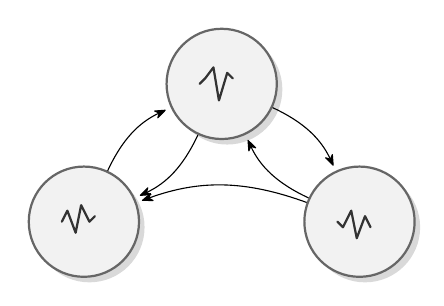
\begin{tikzpicture}[
        scale=0.7,
        % Global Styles
        >={Stealth[round, sep=2pt]}, % Arrow style
        node_base/.style={
            circle,
            draw=black!60,
            thick,
            minimum size=1.4cm,
            inner sep=0pt,
            fill=gray!10, % All nodes are now grey
            drop shadow={opacity=0.3, shadow xshift=2pt, shadow yshift=-2pt}
        },
        % Style for the waveform lines inside nodes
        wave/.style={thick, black!80, line cap=round, line join=round}
    ]
    
        % --- Define 5 Nodes in a new arrangement (Pentagon-like shape) ---
    
        \node[node_base] (n1) at (0, 0) {};       % Top Left
        \node[node_base] (n2) at (5, 0) {};     % Top Right
        \node[node_base] (n3) at (2.5, 2.5) {};     % Far Right
    
        % --- Draw "Dynamic Features" (Waveforms) inside nodes ---
    
        % Node 1 Wave
        \draw[wave] ([xshift=-0.4cm]n1.center) -- ++(0.1, 0.2) -- ++(0.15, -0.4) -- ++(0.1, 0.5) -- ++(0.15, -0.3) -- ++(0.1, 0.1);
    
        % Node 2 Wave
        \draw[wave] ([xshift=-0.4cm]n2.center) -- ++(0.1, -0.1) -- ++(0.15, 0.3) -- ++(0.1, -0.5) -- ++(0.15, 0.4) -- ++(0.1, -0.2);
    
        % Node 3 Wave
        \draw[wave] ([xshift=-0.4cm]n3.center) -- ++(0.1, 0.1) -- ++(0.15, 0.2) -- ++(0.1, -0.6) -- ++(0.15, 0.5) -- ++(0.1, -0.1);
    
        
    
        % --- Draw Connections (New flow pattern) ---
    
        \draw[->] (n1) to[bend left=20] (n3);
        \draw[->] (n2) to[bend left=20] (n3);
        \draw[->] (n3) to[bend left=20] (n1);
        \draw[->] (n2) to[bend right=20] (n1);
        \draw[->] (n3) to[bend left=20] (n2);
    
    
    \end{tikzpicture}
    \end{figure}
    

\paragraph{GAT-GRU.} This architecture represents a "sequential" approach to spatiotemporal modeling, integrating Graph Attention Networks (GATs) \cite{velickovic2018graph} within a Gated Recurrent Unit (GRU) \cite{cho2014learning} framework. As illustrated in Figure~\ref{fig:models_overview} (left), the input features are first projected through a linear layer before entering the spatial block. The GAT layer employs a multi-head attention mechanism (Head $1$ to Head $S$) to dynamically weigh neighbor importance, aggregating these representations via summation $(+)$ followed by an \textit{ELU} activation. This spatially enriched signal is then passed to the GRU layer, which manages temporal dependencies. Finally, the output stack processes the GRU hidden states through a \textit{ReLU} activation and a final Linear layer to generate the prediction.

\paragraph{Graph WaveNet.} Graph WaveNet \cite{Wu2019} represents a "parallel" approach designed to overcome the computational bottlenecks of recurrent structures. As shown in Figure~\ref{fig:models_overview} (right), the architecture is built upon a stack of $p$ layers containing a Gated Temporal Convolutional Network (G-TCN) and a Gated Convolutional Network (GCN) layer. The G-TCN integrates a 1-dimensional causal convolution that handles temporal flow, while the GCN handles the spatial relationships. The G-TCN splits the input into two branches (TCN-a and TCN-b) processed by tanh and sigmoid ($\sigma$) activations, respectively, which are then combined via an element-wise product ($\times$) to control information flow. The output is further processed by a GCN layer and a residual connection (+) to preserve signal depth. Crucially, the model utilizes skip connections from each layer, which are summed (+) and passed through a deep output stack consisting of alternating ReLU activations and linear layers to produce the final output.


\begin{figure}[h]
\caption{Algorithmic architectures of GAT-GRU (left) and Graph WaveNet (right).}\label{fig:models_overview}
% Subfigure (a) - GATGRU
\begin{subfigure}[b]{0.45\textwidth}

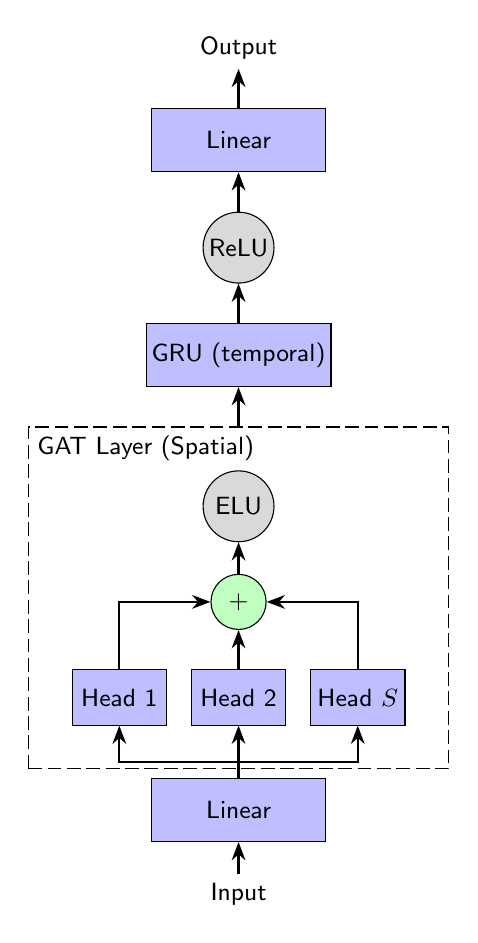
\begin{tikzpicture}[
    % Global Styles (Matched to your WaveNet example)
    font=\sffamily\small,
    >=Stealth,
    % Node Styles
    layer/.style={rectangle, draw=black, fill=blue!25, minimum width=2.2cm, minimum height=0.8cm, align=center, inner sep=2pt},
    small_layer/.style={rectangle, draw=black, fill=blue!25, minimum width=1.2cm, minimum height=0.7cm, align=center, inner sep=2pt},
    act/.style={circle, draw=black, fill=gray!30, minimum size=0.9cm, align=center, inner sep=0pt},
    op/.style={circle, draw=black, fill=green!25, minimum size=0.7cm, align=center, inner sep=0pt},
    % Line Styles
    arrow/.style={->, thick},
    line/.style={thick},
    % Container Styles
    container/.style={draw=black, dash pattern=on 5pt off 2pt, inner sep=0.55cm},
    dotted_box/.style={draw=black, dotted, thick, inner sep=0.2cm}
]

    % ==========================================
    % 1. INPUT
    % ==========================================
    \node (input) at (0,0) {Input};
    \node[layer, above=0.4cm of input] (lin_in) {Linear};
    \draw[arrow] (input) -- (lin_in);

    % ==========================================
    % 2. GAT LAYER (Spatial)
    % ==========================================
    
    % Split point
    \coordinate[above=0.2cm of lin_in] (gat_split);
    \draw[line] (lin_in) -- (gat_split);

    % Attention Heads
    \node[small_layer] (head2) at (0, 2.5) {Head 2};
    \node[small_layer, left=0.3cm of head2] (head1) {Head 1};
    \node[small_layer, right=0.3cm of head2] (head3) {Head $S$};

    % Arrows to heads
    \draw[arrow] (gat_split) -| (head1);
    \draw[arrow] (gat_split) -- (head2);
    \draw[arrow] (gat_split) -| (head3);

    % Aggregation
    \node[op, above=0.5cm of head2] (agg) {+};
    \draw[arrow] (head1) |- (agg);
    \draw[arrow] (head2) -- (agg);
    \draw[arrow] (head3) |- (agg);

    % Activation
    \node[act, above=0.4cm of agg] (elu) {ELU};
    \draw[arrow] (agg) -- (elu);

    % GAT Container
    \node[container, fit=(head1) (head3) (elu), label={[anchor=north west]north west:GAT Layer (Spatial)}] (gat_box) {};

    % ==========================================
    % 3. GRU LAYER (Temporal)
    % ==========================================

    \node[layer, above=0.5cm of gat_box] (gru) {GRU (temporal)};


    % ==========================================
    % 4. OUTPUT STACK
    % ==========================================
    
    \node[act, above=0.5cm of gru] (relu1) {ReLU};
    \node[layer, above=0.5cm of relu1] (lin1) {Linear};
    \node[above=0.5cm of lin1] (final_out) {Output};

    \draw[arrow] (gat_box) -- (gru);
    \draw[arrow] (gru) -- (relu1);
    \draw[arrow] (relu1) -- (lin1);
    \draw[arrow] (lin1) -- (final_out);

\end{tikzpicture}
\label{fig:gatgru}
\end{subfigure}
\hspace{0.1cm}
% Subfigure (b) - WaveNet
\begin{subfigure}[b]{0.45\textwidth}
\centering
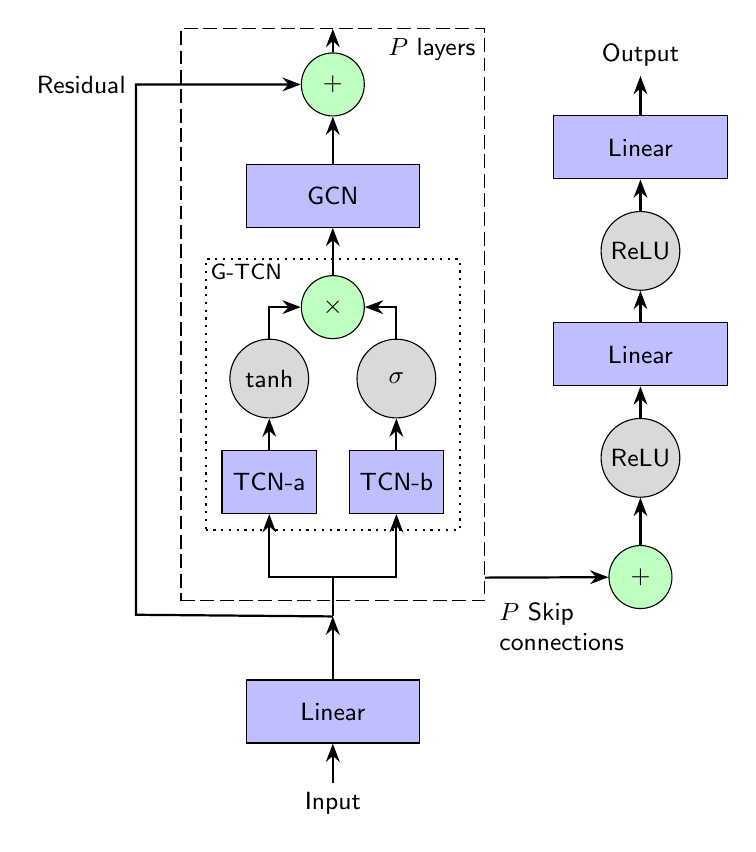
\begin{tikzpicture}[
    % Global Styles
    font=\sffamily\small,
    >=Stealth,
    % Node Styles
    layer/.style={rectangle, draw=black, fill=blue!25, minimum width=2.2cm, minimum height=0.8cm, align=center, inner sep=2pt},
    tcn/.style={rectangle, draw=black, fill=blue!25, minimum width=1.2cm, minimum height=0.8cm, align=center},
    act/.style={circle, draw=black, fill=gray!30, minimum size=1cm, align=center, inner sep=0pt},
    op/.style={circle, draw=black, fill=green!25, minimum size=0.8cm, align=center, inner sep=0pt},
    % Line Styles
    arrow/.style={->, thick},
    line/.style={thick},
    % Container Styles
    container/.style={draw=black, dash pattern=on 5pt off 2pt, inner sep=0.3cm},
    gated_box/.style={draw=black, dotted, thick, inner sep=0.2cm}
]

    % --- 1. Input Section ---
    \node (input) at (0,0) {Input};
    \node[layer, above=0.5cm of input] (lin_in) {Linear};
    \draw[arrow] (input) -- (lin_in);

    % --- 2. The "K Layers" Block ---
    
    % Coordinate for the start of the block
    \coordinate[above=0.8cm of lin_in] (block_start);
    \draw[arrow] (lin_in) -- (block_start);
    
    % Split point for TCNs
    \coordinate[above=0.5cm of block_start] (split_point);
    
    % TCN-a and TCN-b
    \node[tcn, above left=0.8cm and 0.2cm of split_point] (tcna) {TCN-a};
    \node[tcn, above right=0.8cm and 0.2cm of split_point] (tcnb) {TCN-b};
    
    % Arrows to TCNs
    \draw[line] (block_start) -- (split_point);
    \draw[arrow] (split_point) -| (tcna);
    \draw[arrow] (split_point) -| (tcnb);
    
    % Activations
    \node[act, above=0.4cm of tcna] (tanh) {tanh};
    \node[act, above=0.4cm of tcnb] (sigma) {$\sigma$};
    
    \draw[arrow] (tcna) -- (tanh);
    \draw[arrow] (tcnb) -- (sigma);
    
    % Multiply Operation
    \coordinate (mid_act) at ($(tanh)!0.5!(sigma)$);
    \node[op, above=0.5cm of mid_act] (mult) {$\times$};
    
    \draw[arrow] (tanh) |- (mult);
    \draw[arrow] (sigma) |- (mult);
    
    % Gated TCN Container (Dotted Box)
    \node[gated_box, fit=(tcna) (tcnb) (tanh) (sigma) (mult), label={[anchor=north west, inner sep=2pt]north west:\footnotesize G-TCN}] (gated_container) {};

    % GCN Layer
    \node[layer, above=0.6cm of mult] (gcn) {GCN};
    \draw[arrow] (mult) -- (gcn);
    
    % Add Operation (Residual)
    \node[op, above=0.6cm of gcn] (add) {+};
    \draw[arrow] (gcn) -- (add);
    
    % Residual Connection Line
    % Go from block_start, up the left side, to the add node
    \draw[arrow] (block_start) -- (-2.5, 2.4) |- (add) node[pos=0.5, left] {Residual};
    
    % Output of Block
    \coordinate[above=0.3cm of add] (block_out);
    \draw[arrow] (add) -- (block_out);

    % "K Layers" Container (Dash-dotted Box)
    % We draw the "stack" effect first manually behind
    \begin{scope}[on background layer]
        % Main Box
        \node[container, fit=(gated_container) (add) (split_point), label={[anchor=north east]north east:$P$ layers}] (main_box) {};
    \end{scope}

    % --- 3. Skip Connections & Output Stack ---
    
    % Sum Node
    \node[op, right=3.5cm of split_point] (skip_sum) {+};
    
    % Arrows representing skip connections
    \draw[arrow] ($(main_box.south east)+(0.0, 0.3)$) -- (skip_sum);
    \node[below=-0.2cm of skip_sum, xshift=-1cm, align=left] {$P$ Skip\\connections};

    % Output Stack
    \node[act, above=0.6cm of skip_sum] (relu1) {ReLU};
    \node[layer, above=0.4cm of relu1] (lin1) {Linear};
    \node[act, above=0.4cm of lin1] (relu2) {ReLU};
    \node[layer, above=0.4cm of relu2] (lin2) {Linear};
    \node[above=0.5cm of lin2] (final_out) {Output};

    % Connections
    \draw[arrow] (skip_sum) -- (relu1);
    \draw[arrow] (relu1) -- (lin1);
    \draw[arrow] (lin1) -- (relu2);
    \draw[arrow] (relu2) -- (lin2);
    \draw[arrow] (lin2) -- (final_out);

\end{tikzpicture}
\label{fig:wavenet}
\end{subfigure}

\vspace{0.5cm}

% Legend (horizontal, below subfigures)
\centering
\begin{tikzpicture}[
    font=\sffamily\small,
    % Node Styles (matching the main figures)
    layer/.style={rectangle, draw=black, fill=blue!25, minimum width=1.2cm, minimum height=0.5cm, align=center, inner sep=2pt},
    act/.style={circle, draw=black, fill=gray!30, minimum size=0.6cm, align=center, inner sep=0pt},
    op/.style={circle, draw=black, fill=green!25, minimum size=0.5cm, align=center, inner sep=0pt},
    legend_box/.style={draw=black, thick, inner sep=0.1cm}
]

    \node[legend_box, label={above:\textbf{Legend}}] {
        \begin{tabular}{c@{\hspace{0.3cm}}l@{\hspace{0.8cm}}c@{\hspace{0.3cm}}l@{\hspace{0.8cm}}c@{\hspace{0.3cm}}l@{\hspace{0.3cm}}c@{\hspace{0.3cm}}l@{\hspace{0.3cm}}c@{\hspace{0.3cm}}l}
            % Layer/Module
            \begin{tikzpicture}[baseline=-0.5ex]
                \node[layer, minimum width=0.8cm, minimum height=0.4cm] {};
            \end{tikzpicture} & Layer/Module &
            % Activation
            \begin{tikzpicture}[baseline=-0.5ex]
                \node[act, minimum size=0.5cm] {};
            \end{tikzpicture} & Activation &
            % Addition
            \begin{tikzpicture}[baseline=-0.5ex]
                \node[op, minimum size=0.4cm] {+};
            \end{tikzpicture} & Addition &
            % Multiplication
            \begin{tikzpicture}[baseline=-0.5ex]
                \node[op, minimum size=0.4cm] {$\times$};
            \end{tikzpicture} & Element-wise Product
        \end{tabular}
    };

\end{tikzpicture}


\end{figure}

\section{Modeling the GLSL Maritime Network}\label{sec:Spatiotemporal Graph Modeling}

Our data is composed of AIS-derived origin--destination records spanning from January 2013 to December 2024, and includes only trips where at least one endpoint (origin or destination) is a GLSL port. The data captures vessel movements to, from, and throughout the GLSL maritime corridor. This includes 1,265 non-GLSL ports interacting with 87 GLSL ports. The final data table totals 409,882 trips over the 12-year period, involving 1,352 distinct ports and 7,446 commercial vessels.

\subsection{Problem Definition}\label{subsec:Problem Definition}
We define a graph $\mathcal{G} = (\mathcal{V}, \mathcal{E})$ from this data by adapting ports as nodes and trips as edges. The set of nodes and edges are respectively given by $\mathcal{V} = \{v_1, \ldots, v_n\}$ and $\mathcal{E} \subseteq \mathcal{V} \times \mathcal{V}$. Each datapoint contains characteristics about ports, vessels, and trips. Therefore, we define $X_{f} \in \mathcal{R}^{n\times m}$ and $X_e \in \mathcal{R}^{n^2\times l}$ as the matrices for node and edge features, as well as $A \in \mathcal{B}^{n \times n}$, the adjacency matrix. The dimensions $n$, $m$, and $l$, respectively represent the number of nodes, node features, and edge features.

\begin{table}[h]
  \centering
  \caption{Description of the attributes.}
  \label{tbl:features}
  \begin{tabular}{llp{6cm}}
  \toprule
  \textbf{Level} & \textbf{Attributes} & \textbf{Description}\\
  \midrule
  \multirow{5}{*}{Node} & Inbound flows & Number/volume of incoming trips \\
   & Outbound flows & Number/volume of outgoing trips \\
   & Dwell time & Average time vessels spend at the port \\
   & Deadweight & Sum deadweight tonnage of vessels \\
   & Speed over ground (SOG) & Average speed of vessels entering/leaving the port \\
  \midrule
  \multirow{3}{*}{Edge} & Trip duration (avg) & Average trip duration \\
   & Trip duration (std) & Standard deviation of trip durations \\
   & Trip count & Number of trips on an edge \\
  \bottomrule
  \end{tabular}
\end{table}

It is important to select a set of features that can be useful in a counterfactual framework setting, so that decision-makers can use trained models to simulate the impact of a simulated shock on relevant attributes. For instance, by editing the values of the features shown in Table \ref{tbl:features}, one can simulate port congestion or strikes (dwell time and SOG), load rerouting (deadweight), or closing routes (rebalancing deadweight with in and out flows).

So far, we have defined a master graph $\mathcal{G}$ over the whole aggregated 12-year period. However, in order to predict the next state of the network from recent activity, we need to derive subgraphs $\mathcal{G}(t)$ with $t \in \{1,\dots,T\}$ representing snapshots of the network at time $t$. Therefore, each datapoint $\mathcal{G}(t)$ is a collection $\{X_f(t), X_e(t), A(t)\}$.

\begin{figure}[h]
\centering
\caption{Problem definition.}
\label{fig:problem_definition}
  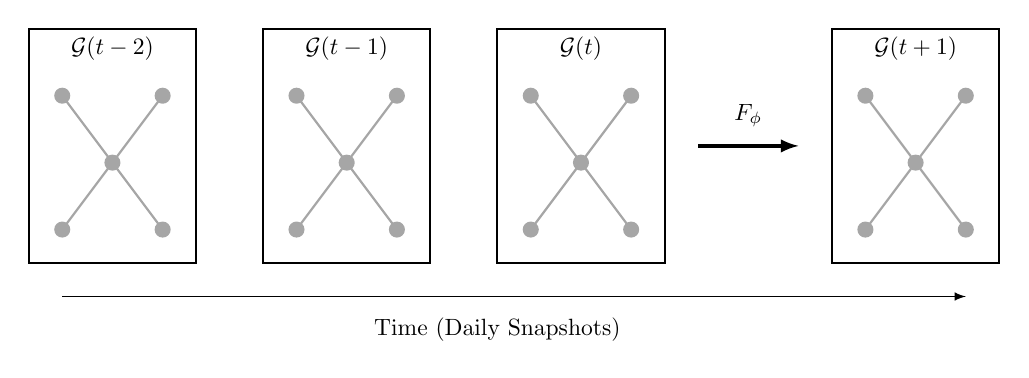
\begin{tikzpicture}[scale=0.85, every node/.style={scale=0.85}]
  
  \foreach \x/\t in {0/t-2, 3.5/t-1, 7/t} {
      \begin{scope}[shift={(\x,0)}]
          \draw[thick] (0,0) rectangle (2.5,3.5);
          \node at (1.25,3.2) {\textbf{$\mathcal{G}(\t)$}};
          
          \foreach \i/\px/\py in {1/0.5/2.5, 2/2/2.5, 3/1.25/1.5, 4/0.5/0.5, 5/2/0.5} {
              \fill[gray!70] (\px,\py) circle (0.12);
          }
          
          \draw[gray!70, thick] (0.5,2.5) -- (1.25,1.5);
          \draw[gray!70, thick] (2,2.5) -- (1.25,1.5);
          \draw[gray!70, thick] (1.25,1.5) -- (0.5,0.5);
          \draw[gray!70, thick] (1.25,1.5) -- (2,0.5);
      \end{scope}
  }
  
  \draw[black, -latex, very thick] (10,1.75) -- (11.5,1.75);
  \node at (10.75,2.2) {$F_{\phi}$};
  
  \begin{scope}[shift={(12,0)}]
      \draw[thick] (0,0) rectangle (2.5,3.5);
      \node at (1.25,3.2) {\textbf{$\mathcal{G}(t+1)$}};
      
      \foreach \i/\px/\py in {1/0.5/2.5, 2/2/2.5, 3/1.25/1.5, 4/0.5/0.5, 5/2/0.5} {
          \fill[gray!70] (\px,\py) circle (0.12);
      }
      
      \draw[gray!70, thick] (0.5,2.5) -- (1.25,1.5);
      \draw[gray!70, thick] (2,2.5) -- (1.25,1.5);
      \draw[gray!70, thick] (1.25,1.5) -- (0.5,0.5);
      \draw[gray!70, thick] (1.25,1.5) -- (2,0.5);
  \end{scope}
  
  \draw[black, -latex] (0.5,-0.5) -- (14,-0.5);
  \node at (7,-1) {Time (Daily Snapshots)};
  
  \end{tikzpicture}
\end{figure}

As depicted in Figure \ref{fig:problem_definition}, we aim to optimize the parameters $\phi$ of a function $F$ that maps the next state of the graph $\mathcal{G}(t+1)$ from a chronological input sequence of graphs $\{\mathcal{G}(t-j), \mathcal{G}(t-j+1), \dots, \mathcal{G}(t)\}$ of length $j$.

At this point, an important consideration arises---time granularity. Indeed, there is a trade-off between time granularity and data sparsity. Some GLSL ports are not very active, and some other non-GLSL nodes rarely interact with the GLSL subnetwork, meaning that the data is inherently sparse. Sparsity naturally increases as $T$ increases.

Unfortunately, time aggregation cannot be used to mitigate sparsity as, for instance, by using weekly snapshots we negatively impact the number of training examples. The proper balance in terms of time granularity depends on the amount of data available, as deep learning models scale with it. In our case, weekly graph snapshots would provide an underwhelmingly small training set, so we instead opt for daily snapshots.

\subsection{Mitigating Sparsity}\label{sec:Mitigating Sparsity}

Using daily GLSL port network snapshots, we obtain a sequence of 4,379 graphs spanning 12 years of activity. A significant challenge in this setting is that the probability of a node showing non-zero feature values on any given day is highly variable. Many ports are structurally present in the master graph but operationally inactive for long periods, acting as "ghost nodes" that introduce noise (zeros) into the training data.

Our sparsity mitigation strategy is twofold: we first apply (a) spatial aggregation to non-GLSL nodes, and then (b) we formulate a temporal filtering algorithm that we apply on the aggregated graphs. Both are needed because (a) alone would fail to eliminate weak signals emanating from mostly inactive ports within the GLSL network, and (b) alone would be too restrictive as most of the exchanges would be pruned as only very few GLSL and international ports interact consistently. This arrangement allows us to eliminate sparsity while preserving most of the information contained in our graph sequence.

\paragraph{Node aggregation.} We create a mapping from port locations to their geographic regions. We divide the world into Oceania, Europe, Asia, Africa, North and South America. The aggregation is applied to non-GLSL nodes since we devise a methodology that focuses on a specific port network. This kind of aggregation reduces the number of nodes as well as the total degree of non-aggregated nodes (the GLSL ports) but significantly increases feature density. This tradeoff works in our favor because the exact location of international partners does not constitute crucial information.

\paragraph{Temporal k-core decomposition.} We mitigate this data sparsity by formulating a k-core decomposition-based algorithm \cite{alvarez2005} that takes temporal availability into account. Our method minimizes sparsity while maximizing coverage under the constraint that the subgraphs must be stable in their structure through time. In other words, we aim to maximize the density of non-zero features while ensuring the resulting subgraph remains structurally cohesive, a prerequisite for the spatial convolution layers in Graph WaveNet.

Algorithm \ref{alg:temporal-kcore} shows how our temporal k-core decomposition algorithm filters nodes based on their connectivity patterns over time. Consider a temporal graph $\mathcal{G} = \{G_1, G_2, \ldots, G_T\}$ where $G_t = (V_t, E_t)$ represents the graph at time $t$. The k-core of a graph $G = (V, E)$ is the maximal subgraph $G_k = (V_k, E_k)$ where each node $v \in V_k$ has degree $\deg(v) \geq k$.

\begin{algorithm}[h]
\caption{Temporal K-Core Decomposition}
\label{alg:temporal-kcore}
\begin{algorithmic}[1]
\Require Temporal graph $\mathcal{G} = \{G_1, \ldots, G_T\}$, k-core parameter $k$, frequency threshold $h \in [0,1]$
\Ensure Filtered node set $V^*$
\State Initialize $\mathcal{A} \gets \{\}$ \Comment{Collection of active node sets}
\For{$t = 1$ to $T$}
    \State $G_t \gets (V_t, E_t)$ \Comment{Get graph at time $t$}
    \If{$k \leq 0$ or $k$ is None}
        \State $A_t \gets V_t$ \Comment{All nodes are active}
    \Else
        \State Remove self-loops from $G_t$
        \State $G_k^t \gets$ K-Core$(G_t, k)$ \Comment{Compute k-core subgraph}
        \State $A_t \gets$ nodes$(G_k^t)$ \Comment{Extract k-core nodes}
    \EndIf
    \State $\mathcal{A} \gets \mathcal{A} \cup \{A_t\}$
\EndFor
\State \Comment{Calculate temporal frequency for each node}
\For{each node $v \in \bigcup_{t=1}^{T} V_t$}
    \State $f(v) \gets \frac{1}{T} \sum_{t=1}^{T} \mathbb{1}_{v \in A_t}$ \Comment{Frequency of $v$ in active sets}
\EndFor
\State $V^* \gets \{v : f(v) \geq h\}$ \Comment{Filter nodes by threshold}
\State \Return $V^*$
\end{algorithmic}
\end{algorithm}

The k-core is the maximal subgraph where each node has at least $k$ connections. For each time step $t$, we compute the k-core decomposition to identify densely connected nodes. We track the frequency $f(v)$ at which each node $v$ appears in the k-core across all time steps. Nodes with frequency $f(v) \geq h$ are retained in the final filtered graph. This identifies ports that maintain strong connectivity patterns over time. The output is a filtered temporal graph dataset compatible with PyTorch Geometric, enabling prediction tasks on maritime traffic patterns.

\subsection{Training and Performance}\label{sec:Training and Benchmarking Graph WaveNet}

After applying Algorithm \ref{alg:temporal-kcore}, we obtain 4,383 temporal graph instances. Input-target sequence pairs were constructed using a sliding window approach with a sequence length of 12 timesteps. For each sequence, the model receives 12 consecutive graph snapshots as input and predicts the graph-level representation of the subsequent timestep. The training process was conducted with the set of hyperparameters described in Table \ref{tab:hyperparameters}.

Figure \ref{fig:losses} illustrates the training dynamics and convergence properties of the three comparative models. All architectures demonstrate stable learning behaviors with monotonic decay in loss after initial stabilization. The LSTM baseline (Figure \ref{fig:losses}(a)) exhibits rapid initial convergence, reaching its best validation loss early at epoch 11. In contrast, the graph-based architectures show distinct behaviors. The GAT-GRU (Figure \ref{fig:losses}(b)) exhibits significant volatility in the initial epochs but stabilizes effectively to achieve a robust descent, reaching its best validation performance at epoch 48. Graph WaveNet (Figure \ref{fig:losses}(c)) converges relatively quickly with its best epoch recorded at 24, though the gap between training and validation loss suggests a higher susceptibility to overfitting compared to the other models. Early stopping (indicated by vertical dotted lines) was deployed to retain the most generalizable weights.

\begin{figure}[h]
\caption{Mean Square Error (MSE) training and validation losses over training epochs given in log scale for LSTM, GAT-GRU and graph WaveNet.}
\label{fig:losses}
\centering
\includegraphics[scale=0.4]{losses_over_epoch.png}
\end{figure}

\begin{table}[h]
\centering
\caption{Comparative performance of temporal graph models on test set. Performance metrics are given in their standardized forms.}
\label{tab:model_comparison}
\begin{tabular}{lccccc}
\toprule
\textbf{Model} & \textbf{MAE} & \textbf{RMSE} & \textbf{Parameters} & \textbf{Training Epochs} & \textbf{Training Time (s)} \\
\midrule
LSTM & $375.41$ & $603.15$ & $88,000$ & $26$ & $1,997$ \\ 
GAT-GRU & $\mathbf{292.20}$ & $\mathbf{435.06}$ & $80,384$ & $50$ & $6,956$  \\ 
WaveNet & $411.83$ & $886.96$ & $221,376$ & $39$ & $5,946$ \\
\bottomrule
\end{tabular}
\end{table}

As shown in Table~\ref{tab:model_comparison}, the GAT-GRU model demonstrates superior performance across both evaluation metrics, achieving the lowest MAE and RMSE on the test set. This represents a significant improvement over the baseline LSTM model and the Graph WaveNet. The enhanced performance of GAT-GRU suggests that the attention mechanisms are successfully capturing the relevant spatial dependencies between nodes, which, when combined with the GRU's temporal processing, yields the most precise predictions. Surprisingly, Graph WaveNet performed the poorest among the three models, with the highest error rates, indicating that its dilated causal convolutions may not have been as effective for this specific dataset configuration compared to the attention-based approach.

Regarding computational efficiency, the models present a trade-off between parameter size, training time, and accuracy (see Table~\ref{tab:model_comparison}). The GAT-GRU model possesses the fewest parameters yet requires the longest training time, likely due to the computational complexity of calculating attention scores across the graph structure. Conversely, Graph WaveNet has the highest parameter count and a training time inferior to that of GAT-GRU. The LSTM baseline remains the most computationally efficient option, but lacks the structural understanding of the GAT-based model. However, it is important to note that these results highly depend on hyperparameters, as these models are very sensitive to them. Consequently, results could differ with a different set of hyperparameters or even on a different data distribution, as these models are also very dependent on data. The hyperparameters we used are shown in Table \ref{tab:hyperparameters} in the Appendix. 

The qualitative differences in model performance are further visualized in Figure \ref{fig:inference}. The LSTM model (Figure \ref{fig:inference}(a)) fails to capture the spatial dynamics, producing a flat-line prediction that approximates the mean of the target variable. Graph WaveNet (Figure \ref{tab:model_comparison}(c)), while attempting to model the fluctuations, exhibits excessive variance and noise, leading to the high error rates observed in Table \ref{tab:model_comparison}. In contrast, GAT-GRU (Figure \ref{tab:model_comparison}(b)) successfully tracks the ground truth signal with reasonable fidelity, confirming its status as the optimal choice for this task.

\begin{figure}[h]
\caption{Overall inference accuracy, ground truth against predictions for LSTM, GATGRU and Graph WaveNet.}
\label{fig:inference}
\centering
\includegraphics[scale=0.4]{inference_result_figure.png}
\end{figure}

\section{Discussion}\label{sec:Discussion}

Temporal graph models offers a foundation to further craft useful tools for decision-makers. For instance, it is possible to generate counterfactual predictions based on edited input graph features as shown in Figure \ref{fig:counterfactual}. Editing an input sequence, or in other words, simulating counterfactual scenarios via intervention in the input data, is done by modifying the relevant values in either the node or edge feature matrix, or both. The now edited graph sequence is fed to the trained model which outputs the associated counterfactual prediction for the next period. In the context of maritime traffic, one might want to create shocks on the inbound flows, or dwell time in order to simulate the effect of strikes or speed regulations. 

\begin{figure}[h]
\caption{Visualization of the counterfactual analysis framework}\label{fig:counterfactual}
  \begin{center}
  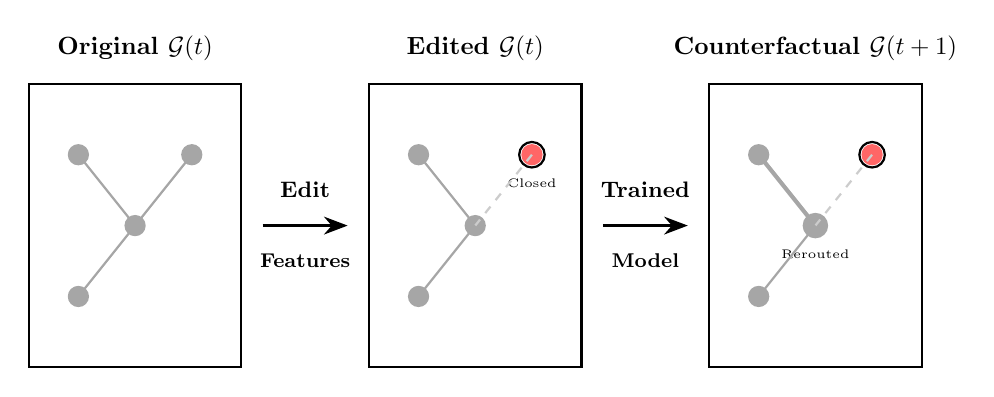
\begin{tikzpicture}[scale=0.9, every node/.style={scale=0.9}]

  \begin{scope}[shift={(0,0)}]
      \draw[black, thick] (0,0) rectangle (3,4);
      \node[black] at (1.5,4.5) {\textbf{Original $\mathcal{G}(t)$}};

      \foreach \i/\px/\py in {1/0.7/3, 2/2.3/3, 3/1.5/2, 4/0.7/1} {
          \fill[gray!70] (\px,\py) circle (0.15);
      }

      \draw[gray!70, thick] (0.7,3) -- (1.5,2);
      \draw[gray!70, thick] (2.3,3) -- (1.5,2);
      \draw[gray!70, thick] (1.5,2) -- (0.7,1);
  \end{scope}

  \draw[-{Stealth[length=3mm]}, black, very thick] (3.3,2) -- (4.5,2);
  \node[black, font=\small] at (3.9,2.5) {\textbf{Edit}};
  \node[black, font=\footnotesize] at (3.9,1.5) {\textbf{Features}};

  \begin{scope}[shift={(4.8,0)}]
      \draw[black, thick] (0,0) rectangle (3,4);
      \node[black] at (1.5,4.5) {\textbf{Edited $\mathcal{G}(t)$}};

      \fill[gray!70] (0.7,3) circle (0.15);
      \fill[red!60] (2.3,3) circle (0.15);
      \draw[black, thick] (2.3,3) circle (0.18);
      \node[black, font=\tiny] at (2.3,2.6) {Closed};

      \fill[gray!70] (1.5,2) circle (0.15);
      \fill[gray!70] (0.7,1) circle (0.15);

      \draw[gray!70, thick] (0.7,3) -- (1.5,2);
      \draw[gray!40, thick, dashed] (2.3,3) -- (1.5,2);
      \draw[gray!70, thick] (1.5,2) -- (0.7,1);

  \end{scope}

  \draw[-{Stealth[length=3mm]}, black, very thick] (8.1,2) -- (9.3,2);
  \node[black, font=\small] at (8.7,2.5) {\textbf{Trained}};
  \node[black, font=\footnotesize] at (8.7,1.5) {\textbf{Model}};

  \begin{scope}[shift={(9.6,0)}]
      \draw[black, thick] (0,0) rectangle (3,4);
      \node[black] at (1.5,4.5) {\textbf{Counterfactual $\mathcal{G}(t+1)$}};

      \fill[gray!70] (0.7,3) circle (0.15);
      \fill[red!60] (2.3,3) circle (0.15);
      \draw[black, thick] (2.3,3) circle (0.18);

      \fill[gray!70] (1.5,2) circle (0.18);
      \node[black, font=\tiny] at (1.5,1.6) {Rerouted};

      \fill[gray!70] (0.7,1) circle (0.15);

      \draw[gray!70, thick, line width=1.5pt] (0.7,3) -- (1.5,2);
      \draw[gray!40, thick, dashed] (2.3,3) -- (1.5,2);
      \draw[gray!70, thick] (1.5,2) -- (0.7,1);

  \end{scope}

  \end{tikzpicture}
  \end{center}
\end{figure}
 
Depending on the input sequence length $j$, it is possible to simulate shocks that propagate over an extensive period of time. However, since $j$ is fixed and defined before training, it is better to know in advance how long the input sequence needs to be. Furthermore, the maximum practical value for $j$ is relative to the total amount of available data points, and excessively long input sequences might hinder training.    

In order to predict for an extended sequence, it is possible to do so by recursively adding the new prediction to the input sequence while respecting the chronological order. It is also possible to train the main model on a larger output sequence, but we advise against it if the number of training examples is not large enough. Indeed, it is significantly more difficult to maintain accuracy as the length of the predicted output sequence increases because of \textit{autoregressive drift} (i.e., error accumulation). Even though Graph WaveNet includes mitigation mechanisms, namely non-autoregressive output and the stacked TCN acting as a feature extractor, the ability to predict long sequences still heavily depends on the training data. 

Structural edits (e.g., closing a port as pictured in Figure \ref{fig:counterfactual}) are possible but more difficult because such intervention needs to be curated also at the edge level, and thus replacing every node feature value of a port by $0$ does not suffice. Also, structural edits must take into account the structure of the model that will be used to predict counterfactual outputs. For instance, if a Graph WaveNet architecture is used, a self-adaptive adjacency matrix is learned from the data during training but the adjacency matrix remains unchanged during test time. Graph WaveNet does not generate a dynamic graph that changes at every time step based on the input features unlike the attention mechanism in GAT, which is dynamic and data-dependent.
 
The lack of cross-validation and model fine-tuning is a limitation of this study. However, we show nonetheless that a priori concepts—such as Graph WaveNet being superior in theory—do not hold all the time, and that GAT-GRU seems the better choice here.

Another crucial consideration is to distinguish between \emph{correlational} and \emph{causal} counterfactuals. The counterfactual predictions that one can generate using the models trained in this study would only reflect learned statistical associations in the training data, not true causal mechanisms. This distinction has important implications for practical applications: while our approach can predict how traffic patterns might change under hypothetical scenarios, it cannot definitively establish whether observed changes would be caused by the interventions or merely correlated with them.

For policy applications—such as evaluating the impact of new port infrastructure or route restrictions—causal inference would be more appropriate. Establishing causality would require either controlled experiments (impractical in maritime contexts) or the application of causal inference frameworks such as do-calculus and structural causal models. Future work should explore integrating these approaches to move beyond predictive counterfactuals toward true causal reasoning.
  

\subsection{Future Directions}
We identify three promising and complementary directions for future research.

First, integrating external data sources is essential for enriching the model context. Supplementing graph data with port capacity databases, trade agreements, cargo manifests, and environmental records would provide crucial information currently missing from purely topological approaches. This integration would support more accurate predictions and grounded counterfactual scenarios.

Second, developing a rigorous causal inference framework using do-calculus and structural causal models would transform correlational counterfactuals into causal interventions. This direction involves identifying confounders, establishing causal graphs, and applying identification strategies to estimate true causal effects from observational data, thereby moving beyond statistical association.

Third, framing the maritime network as an environment for reinforcement learning (RL) could enable the optimization of sequential decisions, such as route planning and capacity allocation, under uncertainty. This approach naturally handles the dynamic, multi-step nature of maritime logistics while learning policies that maximize long-term objectives. These directions are mutually reinforcing: external data integration improves the environment model for RL agents, while causal inference ensures that learned policies reflect true causal mechanisms rather than spurious correlations.

\clearpage

\addcontentsline{toc}{section}{References}

% Bibliography content (from manuscript.bbl)
\providecommand{\href}[2]{#2}\begingroup\raggedright\begin{thebibliography}{10}

\bibitem{Nasiri2017}
M.~Nasiri, B.~Minaei, and Z.~Sharifi, ``Adjusting data sparsity problem using linear algebra and machine learning algorithm,'' \href{http://dx.doi.org/10.1016/j.asoc.2017.05.042}{{\em Applied Soft Computing} {\bfseries 61} (Dec., 2017) 1153--1159}. \url{https://www.sciencedirect.com/science/article/pii/S1568494617303071}.

\bibitem{Li2023b}
Y.~Li, Z.~Li, Q.~Mei, P.~Wang, W.~Hu, Z.~Wang, W.~Xie, Y.~Yang, and Y.~Chen, ``Research on {Multi}-{Port} {Ship} {Traffic} {Prediction} {Method} {Based} on {Spatiotemporal} {Graph} {Neural} {Networks},'' \href{http://dx.doi.org/10.3390/jmse11071379}{{\em Journal of Marine Science and Engineering} {\bfseries 11} no.~7, (July, 2023) 1379}. \url{https://www.mdpi.com/2077-1312/11/7/1379}.

\bibitem{seaway}
``Economic {Impacts}.''
\newblock \url{https://greatlakes-seaway.com/en/the-seaway/economic-impacts/}.

\bibitem{Wu2019}
Z.~Wu, S.~Pan, G.~Long, J.~Jiang, and C.~Zhang, ``Graph {WaveNet} for {Deep} {Spatial}-{Temporal} {Graph} {Modeling},'' \href{http://dx.doi.org/10.48550/arXiv.1906.00121}{{\em arXiv e-prints} (May, 2019) arXiv:1906.00121}. \_eprint: 1906.00121.

\bibitem{velickovic2018graph}
P.~Veli{\v{c}}kovi{\'c}, G.~Cucurull, A.~Casanova, A.~Romero, P.~Li{\`o}, and Y.~Bengio, ``Graph attention networks,'' in {\em International Conference on Learning Representations}.
\newblock 2018.

\bibitem{cho2014learning}
K.~Cho, B.~Van~Merri{\"e}nboer, C.~Gulcehre, D.~Bahdanau, F.~Bougares, H.~Schwenk, and Y.~Bengio, ``Learning phrase representations using rnn encoder-decoder for statistical machine translation,'' in {\em Proceedings of the 2014 Conference on Empirical Methods in Natural Language Processing (EMNLP)}, pp.~1724--1734.
\newblock 2014.

\bibitem{hochreiter1997}
S.~Hochreiter and J.~Schmidhuber, ``Long {Short}-{Term} {Memory},'' \href{http://dx.doi.org/10.1162/neco.1997.9.8.1735}{{\em Neural Comput.} {\bfseries 9} no.~8, (Nov., 1997) 1735--1780}. \url{https://doi.org/10.1162/neco.1997.9.8.1735}.

\bibitem{Wang2022}
S.~Wang, Y.~Lv, P.~Yuan, X.~Piao, and Y.~Zhang, ``Metro {Traffic} {Flow} {Prediction} via {Knowledge} {Graph} and {Spatiotemporal} {Graph} {Neural} {Network},'' \href{http://dx.doi.org/10.1155/2022/2348375}{{\em Journal of Advanced Transportation} {\bfseries 2022} (2022) }. \url{https://login.proxy2.hec.ca/login?url=https://www.proquest.com/scholarly-journals/metro-traffic-flow-prediction-via-knowledge-graph/docview/2720246630/se-2?accountid=11357}.

\bibitem{Huo2024}
G.~Huo, Y.~Zhang, Y.~Lv, H.~Ren, and B.~Yin, ``Urban {Traffic} {Flow} {Forecasting} {Based} on {Graph} {Structure} {Learning},'' \href{http://dx.doi.org/10.1155/atr/7878081}{{\em Journal of Advanced Transportation} {\bfseries 2024} (2024) }. \url{https://login.proxy2.hec.ca/login?url=https://www.proquest.com/scholarly-journals/urban-traffic-flow-forecasting-based-on-graph/docview/3151793912/se-2?accountid=11357}.

\bibitem{Huang2024}
L.~Huang, J.~Qin, and T.~Wu, ``Multisource {Data} {Fusion} {With} {Graph} {Convolutional} {Neural} {Networks} for {Node}‐{Level} {Traffic} {Flow} {Prediction},'' \href{http://dx.doi.org/10.1155/atr/7109780}{{\em Journal of Advanced Transportation} {\bfseries 2024} no.~1, (Jan., 2024) 7109780}. \url{https://onlinelibrary.wiley.com/doi/10.1155/atr/7109780}.

\bibitem{Yuan2025}
X.~Yuan and X.~He, ``Enhancement {Strategy} for {Port} {Resilience}: {Shipping} {Route} {Optimization} {Methods} {Based} on {Network} {Characteristics} of {Ports},'' \href{http://dx.doi.org/10.3390/jmse13020325}{{\em Journal of Marine Science and Engineering} {\bfseries 13} no.~2, (Feb., 2025) 325}. \url{https://www.mdpi.com/2077-1312/13/2/325}.

\bibitem{Yuan2021}
R.~Yan, S.~Wang, L.~Zhen, and G.~Laporte, ``Emerging approaches applied to maritime transport research: {Past} and future,'' \href{http://dx.doi.org/10.1016/j.commtr.2021.100011}{{\em Communications in Transportation Research} {\bfseries 1} (Dec., 2021) 100011}. \url{https://www.sciencedirect.com/science/article/pii/S2772424721000111}.

\bibitem{Liang2022}
M.~Liang, R.~W. Liu, Y.~Zhan, H.~Li, F.~Zhu, and F.-Y. Wang, ``Fine-{Grained} {Vessel} {Traffic} {Flow} {Prediction} {With} a {Spatio}-{Temporal} {Multigraph} {Convolutional} {Network},'' \href{http://dx.doi.org/10.1109/TITS.2022.3199160}{{\em IEEE Transactions on Intelligent Transportation Systems} {\bfseries 23} no.~12, (Dec., 2022) 23694--23707}. \url{https://ieeexplore.ieee.org/document/9868210/}.

\bibitem{Zhang2025}
F.~Zhang, Y.~Wen, O.~Valdez~Banda, M.~Chen, and L.~Du, ``Maritime traffic network extraction and vessel flow prediction in complex inland port clusters,'' \href{http://dx.doi.org/10.1016/j.oceaneng.2025.122791}{{\em Ocean Engineering} {\bfseries 341} (Dec., 2025) 122791}. \url{https://linkinghub.elsevier.com/retrieve/pii/S0029801825024746}.

\bibitem{Zhao2022}
C.~Zhao, X.~Li, M.~Zuo, L.~Mo, and C.~Yang, ``Spatiotemporal dynamic network for regional maritime vessel flow prediction amid {COVID}-19,'' \href{http://dx.doi.org/10.1016/j.tranpol.2022.09.029}{{\em Transport Policy} {\bfseries 129} (Dec., 2022) 78--89}. \url{https://linkinghub.elsevier.com/retrieve/pii/S0967070X22002797}.

\bibitem{scarselli2009graph}
F.~Scarselli, M.~Gori, A.~C. Tsoi, M.~Hagenbuchner, and G.~Monfardini, ``The graph neural network model,'' {\em IEEE Transactions on Neural Networks} {\bfseries 20} no.~1, (2009) 61--80.

\bibitem{wu2021comprehensive}
Z.~Wu, S.~Pan, F.~Chen, G.~Long, C.~Zhang, and S.~Y. Philip, ``A comprehensive survey on graph neural networks,'' {\em IEEE Transactions on Neural Networks and Learning Systems} {\bfseries 32} no.~1, (2021) 4--24.

\bibitem{yu2018spatio}
B.~Yu, H.~Yin, and Z.~Zhu, ``Spatio-temporal graph convolutional networks: A deep learning framework for traffic forecasting,'' in {\em Proceedings of the 27th International Joint Conference on Artificial Intelligence}, pp.~3634--3640.
\newblock 2018.

\bibitem{alvarez2005}
J.~I. Alvarez-Hamelin, L.~Dall'Asta, A.~Barrat, and A.~Vespignani, ``k-core decomposition: a tool for the visualization of large scale networks,'' Oct., 2005.
\newblock \url{http://arxiv.org/abs/cs/0504107}. arXiv:cs/0504107.

\end{thebibliography}\endgroup


\clearpage

\section*{Appendix}

\begin{table}[H]
\centering
\caption{Hyperparameters for the three models}
\label{tab:hyperparameters}
\begin{tabular}{lccc}
\toprule
\textbf{Hyperparameter} & \textbf{LSTM} & \textbf{GAT-GRU} & \textbf{Graph WaveNet} \\
\midrule
\multicolumn{4}{c}{\textit{Training Configuration}} \\
\midrule
Train/Val/Test Split & 0.7/0.15/0.15 & 0.7/0.15/0.15 & 0.7/0.15/0.15 \\
Batch Size & 32 & 32 & 32 \\
Input Sequence Length & 12 & 12 & 12 \\
Number of Epochs & 50 & 50 & 50 \\
Early Stopping Patience & 15 & 15 & 15 \\
\midrule
\multicolumn{4}{c}{\textit{Model Architecture}} \\
\midrule
Hidden Dimension & 64 & 64 & 64 \\
Number of Layers & 2 & 2 (GRU) & 2 (GCN) \\
GAT Layers & --- & 2 & --- \\
Number of Attention Heads & --- & 4 & --- \\
WaveNet Blocks & --- & --- & 4 \\
Layers per Block & --- & --- & 2 \\
Kernel Size & --- & --- & 2 \\
Output Dimension & 64 & 64 & 64 \\
Aggregation & mean & mean & mean \\
Dropout & 0.2 & 0.2 & 0.2 \\
Bidirectional & false & false & --- \\
Use Edge Attributes & --- & false & --- \\
\midrule
\multicolumn{4}{c}{\textit{Optimization}} \\
\midrule
Learning Rate & 0.0001 & 0.0001 & 0.0001 \\
Weight Decay & 0.0001 & 0.00001 & 0.0001 \\
Loss Function & MSE & MSE & MSE \\
Optimizer & Adam & Adam & Adam \\
Gradient Clipping & 1.0 & 1.0 & 1.0 \\
\midrule
\multicolumn{4}{c}{\textit{Learning Rate Scheduler}} \\
\midrule
Use Scheduler & true & true & true \\
Scheduler Type & plateau & plateau & plateau \\
Scheduler Factor & 0.5 & 0.5 & 0.5 \\
Scheduler Patience & 5 & 5 & 5 \\
Scheduler Step Size & 20 & 20 & 20 \\
\bottomrule
\end{tabular}
\end{table}

\end{document}